\subsection{Эксперимент 3. Сравнение SGD и GD.}
\subsubsection{Дизайн эксперимента}
Для сравнения двух методов бралось множество оптимальных параметров, подобранных в предыдущих экспериментах, а именно:
\begin{itemize}
	\item Для GD:
	\begin{enumerate}
		\item $\alpha = 0.1$
		\item  $\beta = 0.01$
		\item  $\omega_0 = 0 \in \mathbb{R}^D$
	\end{enumerate}
	\item Для SGD:
	\begin{enumerate}
		\item $\alpha = 0.1$
		\item  $\beta = 0.0347$
		\item  $\omega_0 = 0 \in \mathbb{R}^D$
		\item  $batch\_size = 10000 $
	\end{enumerate}
\end{itemize}

Далее исследовались методы GD и SGD с данными параметрами по $accuracy$, времени и значению функции потерь.

\subsubsection{Результаты эксперимента}
\begin{figure*}[h]
	\begin{subfigure}{.5\textwidth}
		\centering
		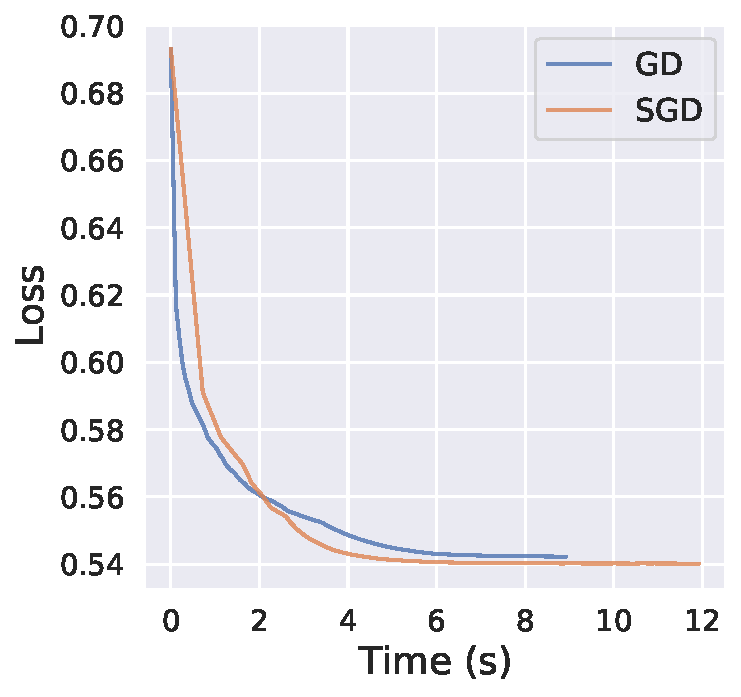
\includegraphics[width=\linewidth]{./experiment3/loss_time.pdf}
		\caption{}
	\end{subfigure}%
	\begin{subfigure}{.5\textwidth}
		\centering
		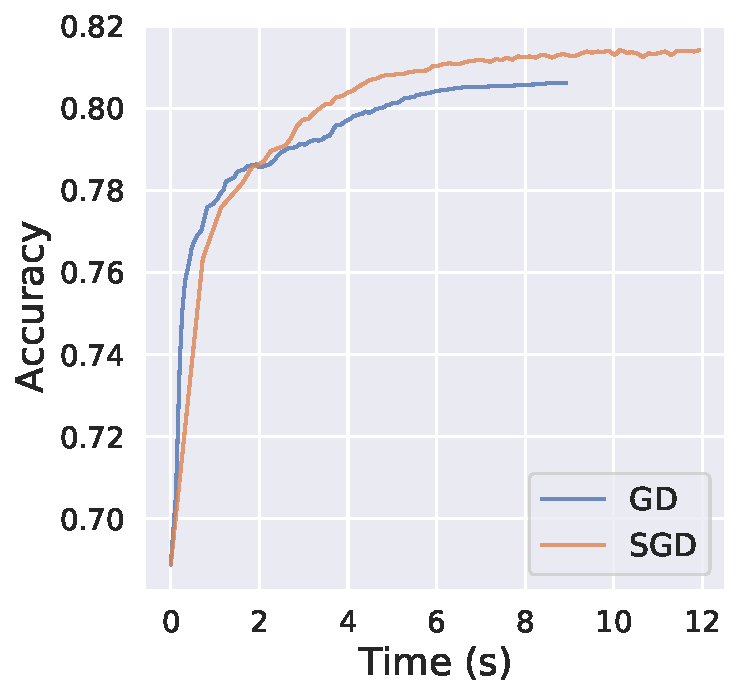
\includegraphics[width=\linewidth]{./experiment3/acc_time.pdf}
		\caption{}
	\end{subfigure}
\caption{}\label{eq:exp3_fig1}
\end{figure*}

\begin{tabular}{|c|c|c|c|}
	\hline
	\multicolumn{4}{|c|}{Сравнение методов}\\
	\hline
		Название  градиентного метода & Время (с)  & Лосс & $accuracy$ \\
	\hline
	  GD & 8.925143 &  0.542243 & 0.806100 \\
	\hline
	  SGD & 11.928005 & 0.540191 & 0.814100 \\
	\hline
\end{tabular}\\


Из рис.\ref{eq:exp3_fig1} и таблицы  видно, что по точности и качеству оптимизации с точки зрения близости к минимуму, а не времени качественно лучше стохастический градиентный спуск. Вычислительная сложность для GD будет $O(N*D*max\_iters)$, а для SGD $O(N*D*max\_iters* \lceil \frac{N}{batch\_size}\rceil)$\footnote{$max\_iters$ для SGD это количество эпох}, поэтому не удивительно, что работать SGD будет дольше.
\subsubsection{Выводы эксперимента}
По качеству наилучшим методом оказался SGD, но по времени он проигрывает GD. При этом с уменьшением размера батча время работы SGD будет увеличиваться обратно пропорционально.

